\section{前言}

隨著智慧型機器人與人工智慧的蓬勃發展,近年來各國均投入於無人載具之開發與研究,已經在非常多場域漸漸出現。在有結構性的環境(structured environments)下,無人駕駛車在從室外之高速公路、郊外人車較少之公路,到室內工廠物流運輸機器人系統已經有相當成熟的發展,其原因在於其所產生的應用是非常貼切人類的日常生活,例如:交通工具、商業物流等。

\begin{figure}[t]
  \centering
    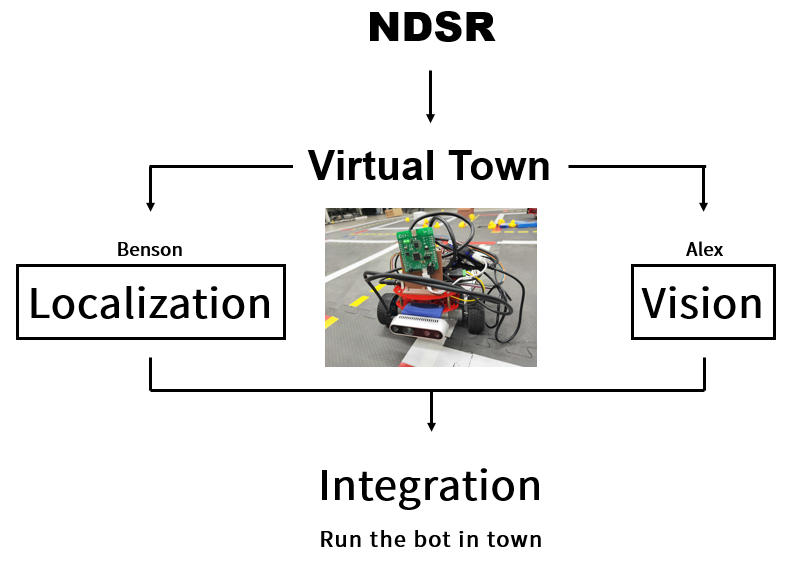
\includegraphics[width=\columnwidth]{images/teaser.png}
        \caption{本計畫目標為建置整合可部署(deployable)無人載具之軟硬體系統,從虛擬環境與微小化平台設計,開發地形與障礙物建模與定位避障導航進行演算法,最後部署於地面與水面無人載具進行實際場域驗證。}
 \label{figure:teaser}
\end{figure}

國防科技一直以來是各個國家的發展重點,有別於在結構性的環境的自動駕駛,非結構性地形(unstructured rough terrain)運作的機器人則包括:緊急搜救機器人、太空/極地探險機器人、軍事野外機器人。美國國防高等研究計劃署 (Defense Advanced Research Projects Agency, DARPA)以及美國太空總署(NASA)針對這樣的挑戰, 舉辦相關競賽,如:2013年DARPA Robotics Challenge以及2017年的Space Robotics Challenge,機器人主要任務就是必須在未知、險惡、無結構性的環境中移動並實現定位、感測、點到點的路徑規劃等功能,在沒有GPS的情況下的進行狀態評估(State Estimation),在不同3D結構中移動、運作而不碰撞,因此一個即時且穩定度高感測系統,以及適合機器人機械設計的運動規劃是非常必要的。

\begin{figure*}[tb]
	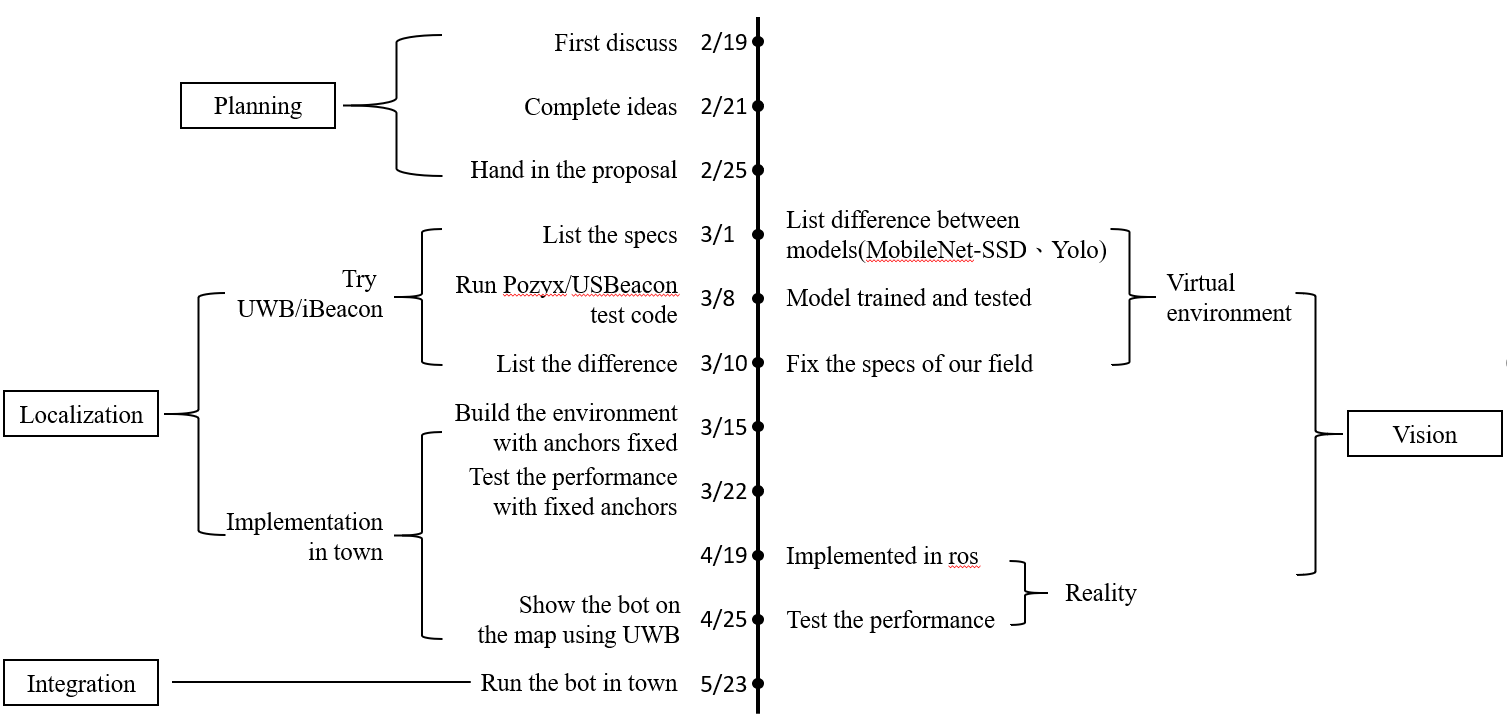
\includegraphics[width=1.8\columnwidth]{images/sys-architecture.png}
	\centering
	\caption{使用ROS (Robot Operating System)之定位任務系統架構}
	\label{figure:localization_sys_architecture}
\end{figure*}

將水面無人載具與國防科技進行實際結合和應用也是各國國防科技重點,在1990年代美國便已開發出可自主探索並監測環境的水面無人載具,隨後在2000年代和法國與新加坡合作開發出無人水面偵查艇,同時, 以色列、英國、德國也投入資源發展裝載測傳感設備且可精準航行和導航的無人水面偵查艇、無人駕駛靶船、無人快速攻擊艇,執行各式水上任務,此時的系統便需要更完整的軟硬體系統整合,且需要一套擁有智慧的判斷系統,在各種軍事情況發生時來進行反應。水面無人載具投入於軍事應用時,較能減少人力的損耗、人為的失誤操作,並能較快速且更有系統去呈現模擬、演習、與實戰。

綜合上述,無人載具需具備立體視覺整合系統感知偵測規則或非規則地形與障礙物,需考量安全、效率等計算出最適合之路徑與運動控制估測進行地面無人載具從A點到B點的運動規劃與移動任務,因此,本論文的目標與貢獻如下:

演算法開發(第一到三季重點):
\begin{enumerate}
\item
機器人模型於Gazebo虛擬平台之建置
\item 
分析點雲及開發演算法於地形與障礙物建模
\item 
開發定位導航任務之運動規劃
\end{enumerate}

實際場域驗證(計畫期末重點)包括:崎嶇地形驗證:戶外斜坡/草地/道路之沿路自主導航測試、水面機器人避障自主導航測試並結合RobotX機器人競賽。

\section{文獻回顧}

\subsection{地形建模、避障與導航}

地形與障礙物建模為實現無人載具在地面或水面自主移動的重要技術,特別在非結構化的環境,建立緊密地圖 (Dense Mapping) 變得必要,為機器人避障/路徑規劃等依據,緊密地圖儲存的模型有:立體像素網格(Voxel Grid)、曲面元素模型(Surfel Model)等,根據不同的儲存空間或運算需求,建立資料結構。MIT開發的Atlas機器人所使用的Kintinuous演算法~\cite{whelan2012kintinuous}, 使用了截斷有符號距離函數(Truncated Signed Distance Function, TSDF) 來產生立體像素網格的資料格式。立體像素網格在實作上採用八元樹(Octree)資料結構進行快速的存取。CHIMP機器人~\cite{stentz2015chimp}同樣也是採用立體像素網格根據不同任務調整解析度,使得機器人在高解析度與計算限制作平衡。RHex~\cite{bogdan2009leaving}則是自行設計一個地圖呈現模式,稱為混和模型 (Hybrid Model)。此模型把地面用多角形呈現、有高度的區域用點來呈現。LAGR機器人~\cite{gerkey2008planning}考量到計算限制在戶外仍然使用簡易的2D佔據柵格(Occupancy Grid),標示地形為自由空間、障礙物等等。Momaro機器人 ~\cite{droeschel2017continuous} 設計多解析度的地圖(Multi-Resolution Map)來儲存,靠近機器人的地圖解析度較高,遠離的則較低。這樣的設計使機器人可以在要與環境互動的區域感測得很清楚,遠處則是大約的規劃未來路徑。

為了讓機器人在環境建模的同時也掌握目前的位置,如何結合不同感測器的觀察結果便成為機器人領域中十分重要的一環,此研究領域又被稱為感測器融合 (Sensor Fusion)。感測器融合主要以機率的方式來實踐,如:卡爾曼濾波 (Kalman Filter)~\cite{gutmann2002markov}、 Information Filter, 連續蒙特卡羅方法 (Sequential Monte Carlo Methods)~\cite{thrun2001robust}。卡爾曼濾波是一個遞迴線性預估器,它藉由連續的觀察與狀態建立出一個線性的統計模型,它也藉由觀察的結果去計算結果的變異數與誤差來更新模型。由於都是藉由機率統計的方式來實踐,因此可以迭代用於物體追蹤 (tracking)、定位 (Localization)與導航 (Navigation),但較少實用在製圖 (Mapping),因為它適合用於嚴謹定義的模型;Information Filter可視為卡爾曼濾波的改良,其數學模型卡爾曼濾波完全相同,它不偵測狀態,也不計算變異數,而是藉由資訊狀態變數(information state variables)與資訊矩陣 (information matrices)來實踐,因此計算量減少,使速度變得更快,它適合實用的領域與卡爾曼濾波相同;連續蒙特卡羅方法 (Sequential Monte Carlo Methods)使用已設定權重的樣本參數來模擬遞迴貝氏更新方程式,以此來描述機率分布的特性。蒙特卡羅方法能套用於狀態轉換模型與觀察模型都是非線性時,這是卡爾曼濾波以及Information filter較做不到的,因為它的資料是使用取樣的方式,因此它可以用用來描述更廣泛的機率密度函數,但它不適用於高維度的模型,因為要用樣本來描述密度函數的話,樣本數是與模型維度成指數成長的。

以上為感測器融合可視為同步定位與地圖構建 (SLAM)的一部分。SLAM在過去二十年為機器人領域最重要的研究問題之一,將 SLAM演算法分成前、後端。前端包含感測資訊、特徵萃取(feature extraction) 以及資訊連結 (data association) 。而後端包含圖論、幾何、以及機率的數學模型,完整的回顧請參考~\cite{cadena2016past}。

\subsection{RobotX無人載具競賽}

在學術、國防、產業的對水面無人載具的需求下,隸屬於國際無人載具協會(Association for Unmanned Vehicle Systems International, AUVSI)之下的RoboNation組織便從2014年開始舉辦國際無人駕駛水上載具競賽Maritime RobotX Challenge,2014年第一次舉辦共有15所,2016第二次共有13所大學參加,而2018包含~\emph{代表台灣的交通大學Team NCTU}共有20所大學參加,參與的學校皆來各國的頂尖大學,其中不乏美國麻省理工學院、新加坡南洋理工學院、韓國首爾大學、澳洲昆士蘭大學,這個競賽的主要目的是為促進學生對於在水上下的自動駕駛機器人的興趣,以及增加對於系統整合自動化的工程與科學的熱情,並進一步的結合學生、研究機構、產業夥伴三方的資源和人力,共同為水上下的自動駕駛機器人領域貢獻心力,舉例來說,比賽隊伍所使用的船隻便是Marine Advanced Research所提供的自適應性波浪快艇(Wave Adaptive Modular Vessel, WAM-V),透過設計此船隻的感測、計算、及動力完成自動駕駛水面及水下系統(Autonomous Maritime System, AMS)並且餐與競賽。Maritime RobotX Challenge競賽進行的方式則是每次比賽皆會設計數個小任務依序讓隊伍去完成並進行評分,例如:穿越進出口與基本控制、避障、停船任務、及水下物體夾取任務,再挑選出分數較高的隊伍進行半決賽和決賽,而此時的任務便是混合先前的多個小任務而成,舉理來說,要在很多障礙物的干擾下完成自動避障病且停船任務的動作,除了大會設計的任務的完成度評分外,每個參賽隊伍也要將所使用的方法跟整個的比賽心路歷程以論文、社群媒體、比賽期間口頭報告的形式呈現,此部分也會納入隊後的排名依據。接著,將依序介紹比賽中各個小任務的規則、應用、所需之技術、和面臨的難度與挑戰。


